\chapter{剽窃代码收集区}

这个章节主要存放一些从网上剽窃的代码,诸如\href{https://www.zhihu.com/}{知乎},\href{https://tex.stackexchange.com/}{stackexchange}……我会尽量注明代码来源,如果读者要用这些代码,也请注明原始来源,以示尊重,谢谢合作。

\section{\LaTeX{}实现类似中括号的方框}

\note[来源]{\href{https://www.zhihu.com/question/55702781}{\LaTeX{}如何实现类似于中括号的方框?-知乎}}

\begin{latex}
\documentclass{article}
\usepackage{tcolorbox}
\tcbuselibrary{most}
\usepackage{lipsum}

\newtcolorbox{mybox}{%
    freelance,
    breakable,
frame code={%
    \draw[line width = 2pt]
    ([xshift=0.5cm]frame.north west) --
    (frame.north west) --
    (frame.south west) --
    ([xshift=0.5cm]frame.south west);
    \draw[line width = 2pt]
    ([xshift=-0.5cm]frame.north east) --
    (frame.north east) --
    (frame.south east) --
    ([xshift=-0.5cm]frame.south east);
},
    colback=white
}

\begin{document}
\lipsum[4]
\begin{mybox}
\lipsum[4]
\end{mybox}
\lipsum[4]
\end{document}
\end{latex}

\section{脚注的带圈数字解决方案}

\note[来源]{\href{https://www.zhihu.com/question/29557216}{\TeX{}的脚注怎么设置比较合理?-知乎}}

\LaTeX{}默认的脚注是上标数字,如果对字母或数字进行脚注解释,很容易背误解为「幂」,如P$ ^1 $,42$ ^2 $。关于带圈数字有不少解决方案,目前我用得比较舒服的是重庆大学毕业论文模版里的方法\footnote{\href{https://github.com/nanmu42/CQUThesis}{GitHub - nanmu42/CQUThesis: 重庆大学毕业论文LaTeX模板}},优点是带圈数字和\lstinline|\rmfamily|字体一致,但是数字不能超过10。

这里提供的刘海洋的解决方法,数字可以超过10,但是带圈数字字体由ipag.ttf提供,与罗马字族字体不一致。对中文文档,xeCJK将20以内的带圈数字认做西文符号,20以上的带圈数字认做CJK符号,因此需要分别设置字体(或者改变这些符号的类型)。

\begin{latex}
\usepackage{xunicode-addon}
\newfontfamily\fnmarkfont{ipag.ttf} % 带圈 0 到 20 被认做西文符号
\newCJKfontfamily\fnCJKmarkfont{ipag.ttf} % 带圈数字超过 20 是 CJK 符号
\renewcommand\thefootnote{{\fnmarkfont\fnCJKmarkfont\textcircled{\arabic{footnote}}}}
\end{latex}

效果如\autoref{fig:plagiarism-footnote}~所示:

\begin{figure}[!htbp]
    \centering
    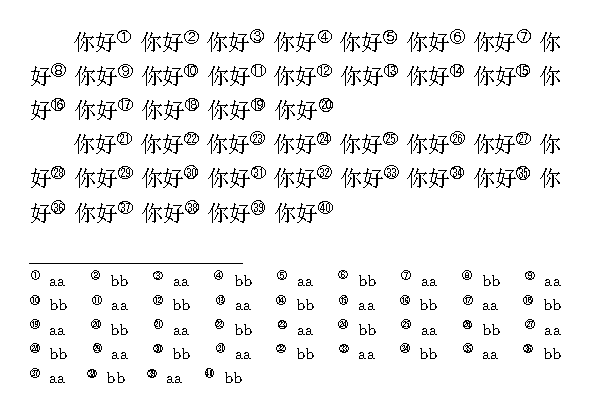
\includegraphics[width=0.8\linewidth]{plagiarism-footnote}
    \caption{带圈脚注示意图}
    \label{fig:plagiarism-footnote}
\end{figure}





